\chapter{Theoretical Formulation}
\label{chap:chapter2}

\section{Governing Equation}
The basic governing equations of single-phase flow comprises mass,
momentum conservation are given below. The energy equation is
neglected because the change in flow properties is taking place in the
isothermal condition.  From the single-phase flow conservation
equation, we will extract the equations for multiphase flow based on
the assumption stated
in\cite{CavitationandBubbleDynamics.1995,Hidalgo2014}.\\

\subsection{Homogeneous bubbly flows}
From homogeneous nucleation, theory
\cite{FundamentalsofCavitation.2004}the microbubbles whose diameter is
smaller than 0.5mm only are considered so that hydrostatic pressure
can be neglected in comparison with surface tension. When the
concentration of the bubbles in the flow exceeds these values the
bubble will have a significant effect on the fluid dynamics of the
suspending liquid.  Then the analyses of the multiphase mixture will
become too complex. In the large context of practical multiphase
flows, one can find a wide range of homogeneities i.e. consisting of
one phase that is very finely dispersed with the other phase of
two-phase flow with a separate stream. The two asymptotic states are
commonly referred to homogeneous and separated flows. They are often
called homogenous mixture flows in the computational domain. The
important aspect of this kind of flow is defining the relative motion
between the two phases because two streams will move in different
velocities and such relative motion between two phases is an implicit
part of the study of separated flow. But based on the assumption, such
as two-phase flows are sufficiently well mixed and the disperse
particle size sufficiently small in order to eliminate any significant
relative motion. Thus the term homogeneous flow some times used to
denote a flow with the relative motion to be zero.  Many bubbly flows
will come close to this approximation. In the absence of relative
motion the governing mass and momentum conservation equations reduce
to a form similar to those for single phase flow.  It is possible to
establish barotropic relation which controls the
condensation$\&$vaporization and this allows one to anticipate that
entire spectrum of phenomena observed in single-phase flow dynamics.

\subsection{Governing equations}
The dynamic model of cavitation is established by using mixture
continuity and momentum equations of RANS turbulence model are stated
below\cite{Zhao2021}.
\begin{equation}
\frac{\partial{{\rho}_m}}{\partial t} + \frac{\partial{{{\rho}_m}
    u_j}}{\partial{x_j}} = 0
\end{equation}

\begin{equation}
\frac{\partial{{\rho}_m}}{\partial t} + \frac{\partial{{{\rho}_m}
    u_j}}{\partial{x_j}}
=\frac{\partial}{\partial{x_j}}\Bigg[{\mu}_m\Bigg(\frac{\partial{u_i}}{\partial{x_j}}+\frac{\partial{u_j}}{\partial{x_i}}\Bigg)\Bigg]
-\frac{\partial}{\partial{x_i}} \Bigg({P}+{\frac{2}{3}}{\mu}_m
\frac{\partial{u_k}}{\partial{x_k}}\Bigg) + {{\rho}_m}g_i
+\frac{\partial{R_{ij}}}{\partial{x_j}}
\end{equation}

\begin{equation}
R_{ij} = {- \rho \overline{{{u_i}^\prime}{{u_j}^\prime}}} = -
\frac{2}{3}\Bigg({\rho}k
+{{\mu}_t}\frac{\partial{u_l}}{\partial{x_l}}\Bigg)\delta{ij} +
{{\mu}_t}\Bigg({{\frac{\partial{u_i}}{\partial{x_j}}}
  +\frac{\partial{u_j}}{\partial{x_i}}}\Bigg) + {\tilde{R_{ij}}}
\end{equation}

The vapour fraction $\alpha$ is used to find density $\rho$ and
dynamic viscosity $\mu$ as shown in eqaution below.
\begin{equation}
\alpha =\frac {\forall{V}}{\forall}
\end{equation}

The mixture density and the viscosity are defined as follows.
\begin{equation}
{{\rho}_m} = {{\rho}_l}{{\alpha}_l} + {{\rho}_v}(1-{{\alpha}_l})
\end{equation}

\begin{equation}
{{\mu}_m} = {{\mu}_l}{{\alpha}_l} +{{\mu}_v}(1-{{\alpha}_l})
\end{equation}

The volume fraction transport equation is given by.
\begin{equation}
\frac{\partial{\alpha}_l}{\partial t}+\frac{\partial}{\partial{x_j}}
({{\alpha}_l}{u_j}) = \frac{\dot{m}}{{\rho}_l}
\end{equation}

\begin{equation}
\dot{m}={{\alpha}_l}\dot{m}^{-} + (1-{{\alpha}_l})\dot{m}^{+}
\end{equation}

\begin{equation}
\frac{\partial{{u_j}}}{\partial{x_j}}=\dot{m}\Bigg(\frac{1}{{\rho}_l}-\frac{1}{{\rho}_v}\Bigg)
\end{equation}

In the above equations, ${\rho}_l$ and ${\rho}_v$ are the liquid and
vapor density, respectively; ${\alpha}_l$ and ${\alpha}_v$ are the
liquid fraction and the vapor fraction, respectively; ${\mu}_m$ is the
mixture laminar viscosity and ${\mu}_t$ is the turbulent viscosity;
and $\dot{m}^+$ and $\dot{m}^-$ represent the condensation and
evaporation rates, respectively.

\section{Basic bubble dynamic equation}
In this simple model\cite{FundamentalsofCavitation.2004}, we consider
the dynamic evolution of the spherical bubble with the fixed center,
which undergoes uniform pressure variation at infinity. This simple
model demonstrates many practical cases such as bubble collapse,
bubble formation from the nucleus, bubble oscillation, etc. Even this
model is suitable for more complicated situations, involving the
motion of the bubble center, which can be approximated by this
model. The liquid motion induced by a spherical cavity in an infinite
medium under the uniform pressure at infinity seems to have been first
considered by Besant in 1859.  It was solved for inviscid liquid by
Rayleigh in 1917, to explain the phenomenon of cavitation erosion. In
1948, Cole use the model of a spherical bubble containing a
non-condensable gas. Plesset in 1954, consider the general case of
bubble evolution for a viscous and non-compressible flow.

\subsection{Assumptions}

\begin{itemize}
\item the liquid is incompressible and either Newtonian or inviscid;
\item gravity is neglected;
\item mass of the air inside the bubble is constant, its inertia is
  neglected. The transformation from one radius to another by the
  bubble take place in isothermal condition;
\item the bubble is saturated with vapor when the local pressure of
  the liquid is well below the vapor pressure.
\end{itemize}

\begin{figure}[H]
 \centering
 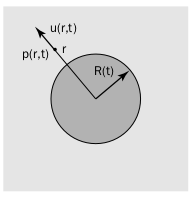
\includegraphics[scale=0.7]{Rayleighplesset.png}
 \caption{Rayleigh Plesset:Evolution of spherical bubble}
  \label{fig:fig13}
\end{figure}

The functions to be determined, in the liquid domain r $\ge$ R(t), are
the velocity u(r,t) and the pressure p(r,t) induced by the evolution
of bubble as shown in (fig2.1).
\subsection{Boundary and intial condition}
In this derivation, we disregard the mass transfer through the
interface, so u(R,t) represents the liquid velocity at the interface
as the interface velocity $/dot R=$$[dR]/[dt]$.  For a viscous fluid
of kinematic viscosity m, the normal stress at the surface is:
\begin{equation}
{t_{rr}}(R,t)=-P(R,t)+2{\mu}{\frac{\partial{u}}{\partial{r}}}\Bigg{\vert}_{r=R}
\end{equation}

The balance normal force is given by:
\begin{equation}
-{t_{rr}}(R,t)=P_{v}+{P_{g}}(t)-{\frac{2S}{R}}
\end{equation}

where $P_g$ stands for the partial pressure of the gas inside the
bubble. With adiabatic gas transformation, the instantaneous gas
pressure is related to the initial gas pressure $P_{g0}$ using the
following expression:
\begin{equation}
{P_{g}}(t)=P_{g0}\Bigg[\frac{R_0}{R(t)}\Bigg]^{3\gamma}
\end{equation}

where $\gamma$ is the ratio of heat gas capacities $C_{pg}$ and
$C_{vg}$.  Thus, the pressure on the cavity interface is given by:
\begin{equation}
P(R,t)=P_{v}+P_{g0}\Bigg[{\frac{R_0}{R(t)}}\Bigg]^{3\gamma}-{\frac{2R}{R}}+2\mu{\frac{\partial{u}}{\partial{r}}}\Bigg{\vert}_{r=R}
\end{equation}

Consider the liquid far from the bubble is assumed to be rest so that
u($\infty$, t)$\rightarrow$0 and the pressure P($\infty$, t) also
denoted $P_{\infty}$(t) is assumed given.  For the initial condition
denoted by the subscript 0, the bubble is assumed to be in
thermodynamic equilibrium, i.e., $\dot{R}$(0), so the equation(1.2) is
satisfied.
\begin{equation}
P_{{\infty}{0}} =P_{g0}+P_v-\frac{2S}{R_0}
\end{equation}

\subsection{Rayleigh-Plesset eqaution}
Based on spherical symmetry, the flow is irrotational and is of the
source type (or sink type). The mass consevation of incompressible
fluid is given by $\triangledown.{\vec{V}}=0$ that gives:
\begin{equation}
u(r,t)=\dot{R}\frac{{R}^2}{{r}^2}
\end{equation}

The viscous term of the Navier-Stokes equation is zero in this
specific case. Thus for both a viscous and non-viscous fluid, the
momentum equation is:
\begin{equation}
{\frac{\partial u}{\partial t}}+u{\frac{\partial u}{\partial r}}=-{\frac{1}{\rho}}{\frac{\partial p}{\partial r}}
\end{equation}

By taking equation(2.15) in to account:
\begin{equation}
{\ddot{R}}{\frac{{R}^2}{r^2}}+2{{\dot{R}}^2}\Bigg[{\frac{R}{r^2}}-{\frac{R^4}{r^5}}\Bigg]=-{\frac{1}{\rho}}{\frac{\partial{p}}{\partial{r}}}
\end{equation}

Integrating with respective to r and considering the condition at
infinity, one can obtains:
\begin{equation}
{\frac{P(r,t)-{P_{\infty}}(t)}{\rho}}={\ddot{R}}{\frac{{R}^2}{r^2}}+2{\dot{R^2}}{\Bigg[{\frac{R}{r}}-{\frac{R^4}{4r^4}}\Bigg]}
\end{equation}

This equation is similar to Bernoulli's equation for a variable
unsteady flow of inviscid liquid. On the other hand when substituting
r=R, equation(2.18) gives:
\begin{equation}
{\frac{P(r,t)-{P_{\infty}}(t)}{\rho}}=R{\ddot{R}}+{\frac{3}{2}}{\dot{R^2}}
\end{equation}

Finally, from the equation(2.13) for the pressure at the interface,
and noting that:
\begin{equation}
{{\frac{\partial u}{\partial r}}\Bigg{\vert}_{r=R}}=-{\frac{2\dot R}{R}}
\end{equation}

equation(2.19) becomes:
\begin{equation}
 {\rho \Bigg[{R{\ddot{R}} + {\frac{3}{2}}{\dot{R^2}}}\Bigg]} = {P_v} -
 {{P_{\infty}}(t)}+{P_{g0}}{\Bigg({\frac{R_0}{R}\Bigg)^{3\gamma}}} -
 {\frac{2S}{R}} - 4\mu{\frac{\dot R}{R}}
\end{equation}

This equation is called the Rayleigh-Plesset equation, which permits
us to determine the temporal evolution of the radius R and
simultaneously the pressure field in the liquid when the law
$P_{\infty}$ is given. For inviscid liquid, the last term on the
right-hand side vanishes. The corresponding equation is known as the
Rayleigh equation.  Both the Rayleigh-Plesset equation and Rayleigh
equation are differential and enormously non-linear, because of the
inertial terms. With the use of the Rayleigh equation, we can solve
the problem of bubble collapse and bubble explosion.  In most
instances, the inertial forces are dominant and viscosity does no
longer plays a huge role. The position of surface tension is often a
secondary case of bubble collapse.

\subsection{Schnerr-Sauer mass transfer model}
According to the detailed literature review, the cavitation model used
in this study was developed by Schneer and Sauser. The Schneer and
Sauser mass transfer cavitation model are derived from a simplified
Rayleigh-Plesset equation which neglects the second-order derivative
of the bubble radius. In reference\cite{Zhao2021, Hidalgo2014}, the
vapor fraction was related to the average radius of the gas nucleus
and number density.  The condensation and evaporation rates are as
follows:
\begin{equation}
{{\alpha}_v}=\frac{{{n}_0}{\frac{4}{3}}\pi{{R}^3}}{\Bigg({n_0}{\frac{4}{3}}\pi{R^3}+1 \Bigg)}
\end{equation}

\begin{equation}
{{\dot m}^+}={C_v}{\frac{{{\rho}_v}{\rho}_l}{\rho}}{{\alpha}_v}{(1-{\alpha}_v)}{\frac{3}{R}}{\sqrt{\frac{2({P_v}-{P})}{3{\rho}_l}}} \\     
({if P<P_v})
\end{equation}

\begin{equation}
 {{\dot{m}}^-}={C_c}{\frac{{{\rho}_v}{\rho}_l}{\rho}}{{\alpha}_v}{(1-{\alpha}_v)}{\frac{3}{R}}{\sqrt{\frac{2({P}-{P_v})}{3{\rho}_l}}}
 \\ ({if P>P_v})
\end{equation}

where ${m}^+$, ${m}^-$ are the condensation and evaporation rate
respectively; $C_v$, $C_c$ are the empirical coefficient for
condensation and evaporation, with the value 2, 1 respectively.\\ The
bubble radius can be related to the vapor volume fraction and the
bubble number density:
\begin{equation}
 R=\Bigg({\frac{{{\alpha}_v}}{1-{{\alpha}_v}}}{\frac{3}{4{\pi}{n_0}}}\Bigg)
\end{equation}

From the equation of radius the parameter $n_0$ is the number of gas
nucleus per unit volume. This is an important parameter and it set as
$1.6 \times 10^{13}$ in this thesis.
  
\section{Introduction to Turbulence}

The majority of flows in engineering application encounters
turbulence\cite{ANSYS}. Therefore appropriately turbulent model should
be essential while dealing with complex turbulence flow problems.  The
main properties of turbulent flows are:

\begin{itemize}
\item High unsteadiness,
\item Three-dimensionality,
\item High diffusivity(turbulent diffusion),
\item Dissipation,
\item Coherent structure,
\item Fluctuations on broad ranges of length and time scales.
\end{itemize}
\subsection{Reynolds-average Navier-Stokes equation}

The Reynolds decomposition of u and p, instantaneous fields are
decomposed into a mean and fluctuating part; referred
from\cite{pope2000,ANSYS}:

\begin{equation}
{u_i}={\overline{u_i}}+{{u_i}^\prime}
\end{equation}

where ${\overline{u_i}}$, ${{u_i}^\prime}$ are the mean and
fluctuating velocity components.  For pressure and other scalar
quantities:

\begin{equation}
\phi ={\overline{\phi}}+{{\phi}^\prime}
\end{equation}

where $\phi$ denotes scalar quantities such as pressure, energy, or
species concentration.  Substituting expression of this form for the
flow variables in to the instantaneous continuity and momentum
equations and taking a ensemble average, yields the ensemble-averaged
momentum equations. The equation written in cartesian tensor form:
\begin{equation}
{{\frac{\partial \rho}{\partial t}}+{\frac{\partial}{\partial {x_i}}}(\rho u_i)}=0
\end{equation}

The ensemble-average momemtum equation is:
\begin{equation}
{{{\frac{\partial}{\partial t}}(\rho u_i)}+{{\frac{\partial}{\partial
        x_j}}(\rho{u_i}{u_j})}}={-{\frac{\partial P}{\partial
      x_i}}+{\frac{\partial}{\partial
      x_j}}{\Bigg[{\mu}\Bigg({{{\frac{\partial u_i} {\partial
              x_j}}+{\frac{\partial u_j}{\partial
              x_i}}-{\frac{2}{3}}{{\delta}_{ij}}{\frac{\partial
              u_l}{\partial
              x_l}}}}\Bigg)\Bigg]+{\frac{\partial}{\partial
        x_j}}\bigg({-}{\rho}{\overline{{{u_i}^\prime}{{u_j}^\prime}}}\bigg)}}
\end{equation}

Equation(2.28)$\&$ Equation(2.29) are called Reynolds-average
Navier-Stokes (RANS) equations. They show resembles with Navier-Stokes
equation only the difference is the velocities and other scalars
quantities are expressed as ensemble-averaged values. An additional
term that is present in the RANS equation represents the effect of
turbulence. This term
$\bigg({-}{\rho}{\overline{{{u_i}^\prime}{{u_j}^\prime}}}\bigg)$ is
called Reynolds stresses. This must be modeled to overcome the closure
problem(the number of unknown variables is inconsistent with the
number of the equations). Different types of turbulence modeling are
being used to model this Reynolds stress term which is an additional
term in the RANS ensemble-momentum equation.

\subsection{k-$\omega$ sst turbulence model}
After a detailed literature review, it is better to use the k $\omega$
sst model for 2D NACA0012 hydrofoil\cite{Zhao2021,ANSYS}. The
shear-stress transport(sst) k-$\omega$ model was developed by Menter
to effectively blend the robust and accurate formulation of the
k-$\omega$ model in the near-wall region with freestream independence
of the k-$\epsilon$ model in the far-field. The sst k-$\omega$ model
is similar to the standard k-$\omega$ model but includes the following
refinements.

\begin{itemize}
\item The standard k-$\omega$ model and the transformed k-$\epsilon$
  model are both multiplied by a blending function and both models are
  added together. The blending function is designed to be one in the
  near-wall region, which activates the standard k-$\omega$ model and
  zero away from the surface, which activates the transformed
  k-$\epsilon$ model.
\item The sst model incorporates a damped cross-diffusion derivative
  term in the $\omega$ equation.
\item The definition of the turbulent viscosity is modified to account
  for the transport of the turbulent shear stress.
\item The modeling constants are different.
\end{itemize}

These features make sst k-$\omega$ model more accurate and reliable
for a wider class of flows such as adverse pressue gradient flows,
airfoil, transonic shock waves, than standard k-$\omega$ model.

\subsection{Transport equation for the sst k-$\omega$ model}
Turbulent kinetic energy equation reads:
\begin{equation}
{{{\frac{\partial {\rho k}}{\partial t}}+{\triangledown \cdot(\rho k
      \overline{u})}}-{\triangledown \cdot
    ({{\Gamma}_{k,eff}}\triangledown{k})}}
   ={min(G,{c_1}{{\beta}^*}k\omega)-{{\beta}^*}k\omega}
\end{equation}

\begin{equation}
{{\Gamma}_{k,eff}}={{{\alpha}_k}{{\mu}_t}}+{\mu}
\end{equation}

Specific dissipation rate equation reads as:
\begin{equation}
{{{\frac{\partial}{\partial t}}(\rho
    \omega)}+{{\triangledown\cdot(\rho \omega
      \overline{u})}}-{\triangledown({{\Gamma}_{\omega,eff}})}} 
    ={{{\gamma}_{min}}\bigg[{S_2},{\frac{c_1}{a_1}}{{\beta}^*}\omega
    max\bigg
    ({a_1},{\omega},{b_1}{F_{2}\sqrt{S_2}\bigg)\bigg]}}
    -{{\beta}{{\omega}^2}+(1-{F_1})CD_{k\omega}}
\end{equation}

\begin{equation}
{{\Gamma}_{\omega,eff}}={{{\alpha}_{\omega}}{{\mu}_t}+{\mu}}
\end{equation}

The eddy viscosity is calculated as:
\begin{equation}
{{\mu}_t}={\frac{{a_1}\rho k}{max\bigg[{a_1}{\omega},
  {b_1}{F_2}\sqrt{2}\bigg\vert{{\frac{1}{2}\bigg({\triangledown \overline{u}}
  +{(\triangledown \overline{u})^{T}}\bigg)\bigg\vert }}\bigg]}}
\end{equation}

and the production of turbulent kinetic energy reads:
\begin{equation}
{G}={{\mu}_t}{S_2}
\end{equation}

\begin{equation}
{S_2}={2\bigg\vert{{\frac{1}{2}\bigg({\triangledown \overline{u}}
  +{(\triangledown \overline{u})^{T}}\bigg)\bigg\vert}^2}}
\end{equation}
The use of k-$\epsilon$ in the freestream removes the sensitivity of
the original k-$\omega$ to the inlet freestream turbulence
properties. The use of k-$\omega$ in the inner parts of the boundary
layer makes the model usable close to the wall without damping
functions. Thus, each of the constant represents a blend of constants
from $set_1$(k-$\omega$) and $set_2$(k-$\epsilon$):
\begin{equation}
{{\alpha}_k}={F_1}({{\alpha}_{k1}}-{{\alpha}_{k2}})+{{\alpha}_{k2}}
\end{equation}

\begin{equation}
{{\alpha}_{\omega}}={F_1}({{\alpha}_{\omega 1}}-{{\alpha}_{\omega 2}})+{{\alpha}_{\omega 2}}
\end{equation}

\begin{equation}
{{\beta}}={F_1}{({{\beta}_1}-{{\beta}_2})}+{{\beta}_2}
\end{equation}

\begin{equation}
{\gamma}={F_1}({{\gamma}_1}-{{\gamma}_2})+{{\gamma}_2}
\end{equation}

where the blending is performed via blending functions, $F_1$ is a
function that is one in the sublayer and logarithmic region of the
boundary layer and gradually switches to zero in the wake region:
\begin{equation}
{F_1}=tanh\bigg[(arg_1)^4 \bigg]
\end{equation}

\begin{equation}
{arg_1}=min\Bigg(min\Bigg[max\Bigg({{\frac{\sqrt{k}}{{{\beta}^*}\omega
        y}},{\frac{500\mu}{\rho
        {y^2}\omega}}\Bigg),{{\frac{4{{{\alpha}_{{\omega {2}}}}{\rho}
            {k}}}{CD_{k \omega +}{y^2}}}}\Bigg],10 }\Bigg)
\end{equation}

$F_2$ is a function that is one for the biundary-layer flows and zero
for free shear layers:

\begin{equation}
{F_2}=tanh\bigg[(arg_2)^2\bigg]
\end{equation}

\begin{equation}
{arg_2}=min\Bigg[max\Bigg({\frac{2 \sqrt{k}}{{{\beta}^*}\omega y}},
  {\frac{500 \mu}{{\rho}{y^2}{\omega}}}\Bigg),100\Bigg]
\end{equation}

positive term of cross-diffusion term is introduced for numerical
stability:
\begin{equation}
{CD_{k \omega +}}=max({CD_{k \omega}},{10}^{-10})
\end{equation}

\begin{equation}
{CD_{k \omega}}={2 \rho {\alpha}_{\omega 2}}{\frac{{\triangledown
      k}\cdot{\triangledown {\omega}}}{\omega}}
\end{equation}

Closure coefficient have the following values: ${{\alpha}_{k1}}=0.85$,
${{\alpha}_{k2}}=1$, ${{\alpha}_{\omega 1}}=0.5$, ${{\alpha}_{\omega
    2}}=0.856$, ${{\beta}_1}=0.075$, ${{\beta}_2}=0.0828$,
${{\beta}^*}=0.09$, ${{\gamma}_1}=5/9$, ${{\gamma}_2}=0.44$,
${a_1}=0.31$, ${b_1}=1$, ${c_1}=10$.

\subsection{Near-wall treatment}
The near-wall area is separated into the inner and outer turbulent
boundary layers when examining a portion of the wall-bounded turbulent
flows. The inner wall is briefly investigated because, all of the key
phenomena for near-wall flow modeling in CFD occur in this
layer. Various regions of the turbulent boundary layer are shown
in(figure2.2)

\begin{figure}[H]
 \centering
 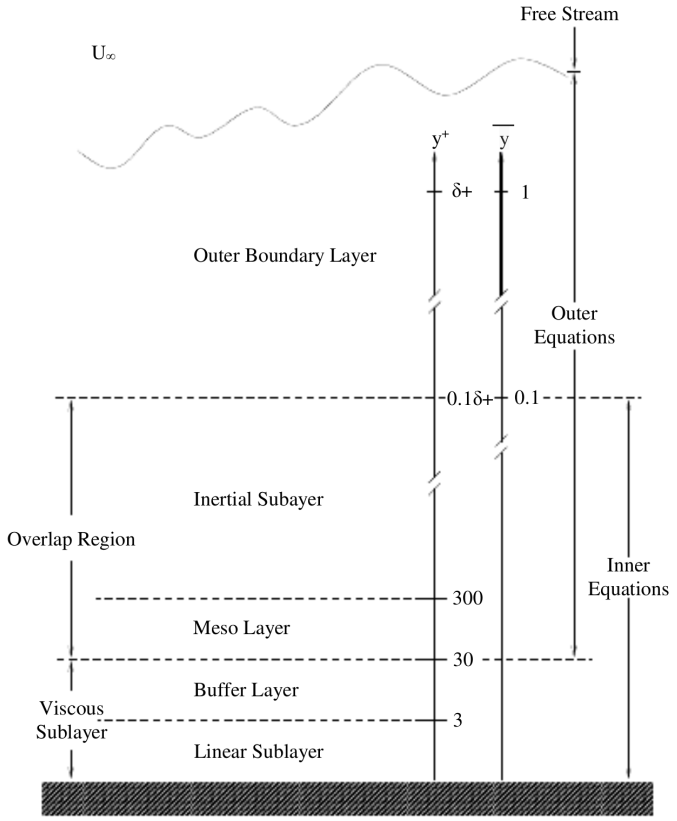
\includegraphics[scale=0.2]{Regionofturbulentboundarylayer}
 \caption{Regions of the turbulent boundary layer}
 \label{fig:fig14}
\end{figure}

From the figure(2.2) the inner layer consists of: the viscous linear
sublayer($0<{y^+}<5$), the buffer sublayer($5<{y^+}<30$) and the
inertial sublayer($30<{y^+}<200-300$) where ${y^+}$ is the normalised
distance tot he wall calculated as:

\begin{equation}
{y^+}={\frac{{{C_{\mu}}^{1/4}}{k^{1/2}}}{\nu}}y
\end{equation}

The molecular viscosity dominates the viscous sub-layer, and
turbulence effects are minimal. The turbulent layer viscosity
dominates the inertial sub-layer, making molecular viscosity
irrelevant.  Both turbulence and molecular viscosity are equally
relevant in the buffer layer. \\

\begin{figure}[H]
 \centering
 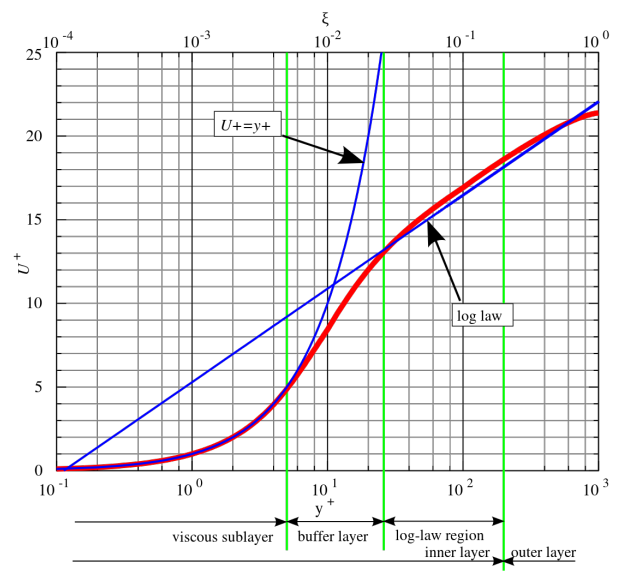
\includegraphics[scale=0.3]{Lawofthewall}
 \caption{Law of the wall}
 \label{fig:fig15}
\end{figure}

The assumptions described allow for the use of simple relations to
represent the behavior of influencing variables in the near-wall
region (as functions of wall distance).  Figure(2.3) depicts the
relationship between dimensionless velocity U + and y +. (the red line
represents the experimental observations and the two blue lines
represent the two derived profiles).  The experimental results were
best suited by the linear profile in the viscous sublayer and the
logarithmic profile in the inertial sublayer, with the buffer sublayer
serving as a smooth transition between the two.  As a result, the
first cell center should be placed in either the viscous linear
sublayer or the inertial sublayer. Because the buffer sublayer
reflects a transition from linear to log, it should be avoided.
Placing the first cell in the linear sublayer is assigned for low
Reynolds turbulence modeling while placing in the inertial(log-layer)
is a characteristic of high Reynolds turbulence modeling. In OpenFOAM
wall function for the field k is denoted with kqRWallFunction, for
field $\omega$ omegaWallFunction and the correction ${\mu}_t$ is done
in nutWallFunction.

\subsection{Automatic wall treatment for k-$\omega$ sst turbulence model}
The equation has a known solution in both the viscous and inertial
(log-layer) sublayers, the k-$\omega$ sst turbulence model does not
require extra damping functions to behave as a low Reynolds model.
Because the $\omega$ equation has a known solution in both viscous and
inertial(log-layer) sublayer. Menter devised a blending technique
based on this feature that enables a smooth shift from high to low
Reynolds formulation and vice versa.  Despite the smooth shift, the
buffer layer is not correctly represented by automatic wall treatment.

\begin{equation}
{\omega}={\sqrt{{{{{\omega}^2}_{vis}}}+{{{{\omega}^2}_{log}}}}}
\end{equation}
where ${\omega}_{vis}$ and ${\omega}_{log}$ are defined as follows:
\begin{equation}
{{\omega}_{vis}}={\frac{6\mu}{{{\beta}_1}{\rho}{y^2}}}
\end{equation}
\begin{equation}
{{\omega}_{log}}={\frac{{k}^{1/2}}{\kappa {{C_{\mu}}^{1/4}} y}}
\end{equation}

The value of $\omega$ for the cell adjacent to the wall is obtained
from eqaution(2.48). In these cells the production term G is given by:
\begin{equation}
G={G_{vis}}   (if {y^+}\le{{{y}^+}_{lam}})
\end{equation}

\begin{equation}
G={{G}_{log}} (if {{y^+}}\ge{{{y}^+}_{lam}})
\end{equation}

\begin{equation}
{G_{vis}}=0
\end{equation}

\begin{equation}
{G_{log}}={\frac{{{C}^{1/4}}_{\mu}
    {{k}^{1/2}}({{\mu}_t}+{\mu})\vert{{\triangledown
        \overline{u}}}\vert}{\kappa y {\rho}}}
\end{equation}
where

\begin{equation}
{{y^+}_{lam}}={\frac{{ln\bigg(max\bigg(E{{y^+}_{lam}},1\bigg)\bigg)}}{\kappa}}
\end{equation}
where E is a dimensional constant with default value of 9.8 and
${y}^+$ from equation(2.47) are calculated.
